\chapter{Lavoro sviluppato} 
\label{Cap3}

\section{Esempio Ambiente Matematico}
\textbf{Def. 3} \textit{Dato un insieme $S$ di coppie che sono un minimo locale di $\epsilon'(p_1,p_2)$, una coppia $(t_a,t_b) \in S$ tale che  $t_a \leq t_i \leq t_j \leq t_b$ e $\mathcal{L} \cap l_{a,b} = \lbrace z(t_a),z(t_b)\rbrace$, dove $l_{a,b}$ Ë la linea retta che unisce $z(t_a)$ e $z(t_b)$.}\\
In tale definizione, la condizione $\mathcal{L} \cap l_{a,b} = \lbrace z(t_a),z(t_b)\rbrace$ indica che la linea $l_{a,b}$ non interseca il contorno esclusivamente in $z(t_a)$ e $z(t_b)$. Si usano solo le prime coppie per calcolare la dimensione deformabile $r$.   

\section{Immagine}
\begin{figure}[h!]	
  \caption{ (a) La distribuzione di $\omega(p,r)$ sul contorno. Più densi sono i "+", più grande é il valore di $\omega(p,r)$}
  \label{contour_2}
  \centering
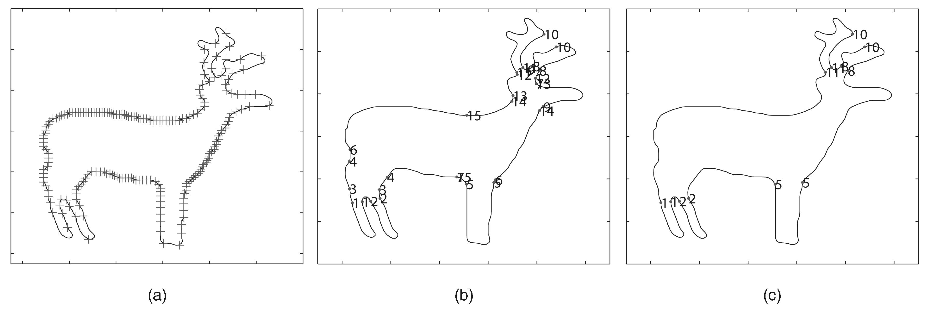
\includegraphics[width=126.48mm, height=42.67mm]{./Figures/contour_flex_deer.png}
\end{figure} 
